\section{Kịch bản Tương tác Người dùng}
    % Tính tiện lợi của sản phẩm được thể hiện qua khả năng tương tác không dây và giao diện quản trị trực quan.

    % \begin{enumerate}
    %     \item \textbf{Cấu hình ban đầu (Provisioning):} 
    %     Người dùng sử dụng điện thoại hoặc máy tính kết nối vào mạng Wi-Fi của Gateway. Một trang Web cấu hình (Captive Portal) sẽ tự động hiện ra, cho phép thiết lập các thông số kết nối chỉ trong vài bước thao tác đơn giản.
        
    %     \item \textbf{Giám sát qua Dashboard tập trung:} 
    %     Khi hệ thống vận hành, người dùng có thể truy cập vào giao diện Dashboard để theo dõi trạng thái hoạt động của từng mô-đun, xem dữ liệu cảm biến hoặc kiểm tra nhật ký (Logs) được lưu trên thẻ nhớ SD.
        
        

    %     \item \textbf{Bảo trì và Cập nhật:} 
    %     Người dùng có thể thực hiện nâng cấp tính năng cho cả hai MCU Master và Slave thông qua tính năng OTA (Over-The-Air) trực tiếp từ giao diện Web, giúp tiết kiệm thời gian và công sức bảo trì tại hiện trường.
    % \end{enumerate}

    Tính tiện dụng của sản phẩm được thể hiện qua khả năng tương tác linh hoạt với các mô-đun/giao thức và giao diện quản trị trực quan. Người dùng (kỹ thuật viên hoặc quản trị viên) tương tác với hệ thống thông qua các kịch bản chính sau:

    \subsection{Cấu hình ban đầu bằng Ứng dụng PC}
    Đây là kịch bản dành cho kỹ thuật viên triển khai tại hiện trường, sử dụng App cấu hình trên PC kết nối với gateway qua cổng USB-C. Ứng dụng hỗ trợ đa giao thức (UART/USB CDC) và cung cấp giao diện đồ họa. Quy trình thác tác tiêu chuẩn gồm:

    \begin{itemize}
        \item \textbf{Quét và nhận diện:} App tự động phát hiện gateway khi kết nối cáp và xác nhận thiết bị sẵn sàng.
        \item \textbf{Đọc cấu hình:} App tải toàn bộ thông số hiện tại từ gateway để hiển thị lên giao diện.
        \item \textbf{Chỉnh sửa tham số:} Người dùng thác tác trên giao diện dạng biểu mẫu (form) để thiết lập. Hỗ trợ tải lên file JSON preset để provisioning hàng loạt cho nhiều gateway cùng loại stack mô-đun.
        \item \textbf{Ghi cấu hình:} Sau khi nhấn "Apply", App gửi lệnh xuống gateway. Firmware thực hiện validate, lưu NVS và áp dụng cấu hình mới tức thì. Nếu tham số thuộc về LAN-MCU, WAN-MCU sẽ đóng vai trò cầu nối để chuyển tiếp cấu hình.
    \end{itemize}

    \subsection{Cấu hình qua Web Config Portal}
    Khi không có máy tính với App PC, người dùng có thể cấu hình gateway thông qua Web Config Portal tích hợp sẵn:
    \begin{enumerate}
        \item Bật chế độ Web Config Portal (nhấn nút vật lý hoặc qua lệnh Cloud).
        \item Gateway khởi tạo điểm truy cập Wi-Fi (AP mode) phát SSID dạng \texttt{GW-XXXXXX} và kích hoạt mDNS (\texttt{gateway.local}).
        \item Người dùng kết nối điện thoại/máy tính vào SSID đó; trình duyệt tự động chuyển hướng (captive portal) đến giao diện cấu hình Web.
        \item Người dùng nhập các thông số cần thiết (Wi-Fi, Server, v.v.) và nhấn \textit{Lưu}.
        \item Gateway xác thực, lưu NVS, reset và kết nối lại với cấu hình mới.
    \end{enumerate}
    Phương thức này đặc biệt hữu ích cho việc \textit{provisioning} thiết bị mới tại hiện trường mà không cần mang theo laptop.

    % Placeholder for image
    % \begin{figure}[h]
    %     \centering
    %     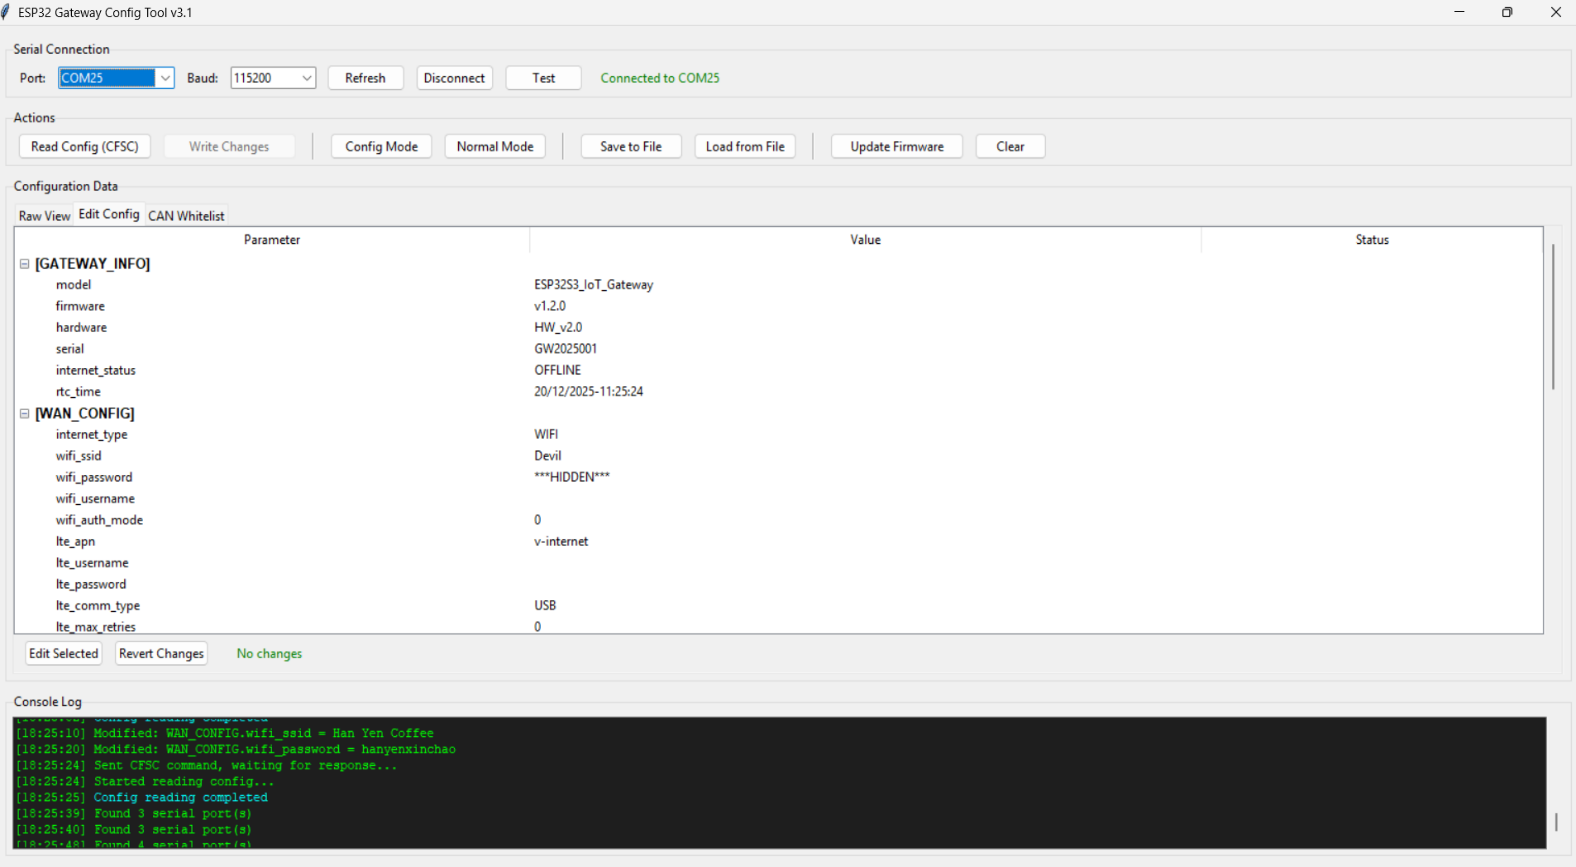
\includegraphics[width=\textwidth]{figures/trienkhai_appconfig.png}
    %     \caption{App config trên PC}
    %     \label{fig:app_config}
    % \end{figure}

    \subsection{Giám sát vận hành qua Giao diện Web (Dashboard/Status)}
    Người quản trị hệ thống giám sát hoạt động của gateway từ xa thông qua Dashboard trên nền tảng Cloud/Web.

    \begin{itemize}
        \item \textbf{Điều kiện bình thường:} Dữ liệu từ các sensor node (thông qua LAN-MCU) được WAN-MCU đưa vào hàng đợi (publish queue) và gửi lên broker/server qua MQTT. Giao diện WAN đang hoạt động (bao gồm trạng thái Internet Monitor) được báo cáo lên Dashboard. Pipeline xử lý này tách biệt luồng \textit{nhận dữ liệu} và \textit{gửi Cloud}, giúp tránh nghẽn cổ chai khi mạng chập chờn.
        \item \textbf{Xử lý sự cố kết nối:} Khi mất kết nối WAN, cơ chế Internet Monitor tự động chuyển đổi sang giao diện dự phòng (Auto-failover). Nếu mất kết nối kéo dài, khối Data Storage Handler sẽ chuyển sang lưu trữ dữ liệu tạm thời vào thẻ nhớ microSD, đảm bảo không mất mát dữ liệu (zero data loss) và tự động đồng bộ lại khi kết nối được khôi phục.
    \end{itemize}

    \subsection{Bảo trì và Cập nhật từ xa (OTA)}
    Trong giai đoạn vận hành và bảo trì, người dùng có thể nâng cấp tính năng hoặc vá lỗi cho cả hai vi điều khiển (Master và Slave) thông qua tính năng OTA trực tiếp từ giao diện Web quản trị.

    \begin{itemize}
        \item Quy trình này giúp tiết kiệm đáng kể thời gian và chi phí đi lại so với việc nạp code thủ công tại hiện trường.
        \item Trong phiên bản 1.0.0, LAN-MCU được cập nhật qua cơ chế \textbf{Wi-Fi NAT}: WAN-MCU khởi tạo điểm truy cập Wi-Fi (NAT mode), LAN-MCU kết nối vào đó và tải gói firmware trực tiếp — cải thiện đáng kể băng thông so với phương thức PPP qua UART của phiên bản nguyên mẫu.
        \item Cơ chế cập nhật được thiết kế ưu tiên tính an toàn: kiểm tra toàn vẹn dữ liệu (checksum/signature), cập nhật tuần tự từng MCU và có cơ chế khôi phục (rollback) nếu quá trình cập nhật gặp lỗi, đảm bảo hệ thống luôn trong trạng thái có thể khởi động được.
    \end{itemize}